\documentclass[5p,times,authoryear]{elsarticle}

\usepackage[authoryear,round]{natbib}
\usepackage{lineno,hyperref}
\usepackage{amsmath,amssymb,amsfonts}
\usepackage{graphicx}
\usepackage{booktabs}
\usepackage{multirow}
\usepackage[hyphens]{url}
\usepackage{float}
\usepackage{placeins}
\def\UrlBreaks{\do\/\do-\do.\do@}

%% --- S-prefix for all figure and table numbering ---
\renewcommand{\thefigure}{S\arabic{figure}}
\renewcommand{\thetable}{S\arabic{table}}
\renewcommand{\thesection}{S\arabic{section}}

\journal{Computers and Chemical Engineering}
\bibliographystyle{elsarticle-harv}

\begin{document}

\begin{frontmatter}

\title{Supplementary Material for: Analyzing Degradation and Extending Life of Electric Vehicle Batteries using Physics-Aware Transformers}

\author[uvce]{Sushanth Chandrashekar}
\author[ese]{Sarina Uke}
\author[iitd1,iitd2,iitd3]{Hariprasad Kodamana\corref{cor1}}
\ead{hkodamana@iitd.ac.in}
\author[iitd1,iitd2]{Manojkumar Ramteke\corref{cor1}}
\ead{mcramteke@chemical.iitd.ac.in}

\cortext[cor1]{Corresponding author}

\affiliation[uvce]{organization={Department of Computer Science and Engineering, Bangalore University},
            city={Bangalore},
            country={India}}

\affiliation[ese]{organization={Department of Energy Science and Engineering, Indian Institute of Technology Delhi},
            city={New Delhi},
            country={India}}

\affiliation[iitd1]{organization={Department of Chemical Engineering, Indian Institute of Technology Delhi},
            city={New Delhi},
            country={India}}
\affiliation[iitd2]{organization={Yardi School of Artificial Intelligence, Indian Institute of Technology Delhi},
            city={New Delhi},
            country={India}}
\affiliation[iitd3]{organization={ANSK School of IT, Indian Institute of Technology Delhi},
            city={New Delhi},
            country={India}}

\end{frontmatter}

This document provides supplementary figures and tables referenced in the main manuscript. All figures are numbered Figure~S1--S7 and tables are numbered Table~S1, corresponding to the references used in the main text.

%% ============================================================
%% S1. TRAINING DYNAMICS
%% ============================================================

\section{Training Dynamics}
\label{sec:S_training}

\subsection{HERO Training Dynamics}

Figure~\ref{fig:S_hero_training} shows the training and validation loss together with the SOH mean absolute error (MAE) over 200 training epochs for the HERO encoder-retrieval model. The bidirectional GRU encoder and cross-attention fusion head were jointly trained using the AdamW optimizer (learning rate 0.001, batch size 64) on 3,979 degradation trajectories from five datasets. The MSE loss drops rapidly in the first 30 epochs as the GRU learns compact trajectory fingerprints, then converges smoothly below 0.10. Validation and training curves track closely throughout, confirming that the retrieval-augmented architecture does not overfit to the training chemistries.

\begin{figure}[!htb]
\centering
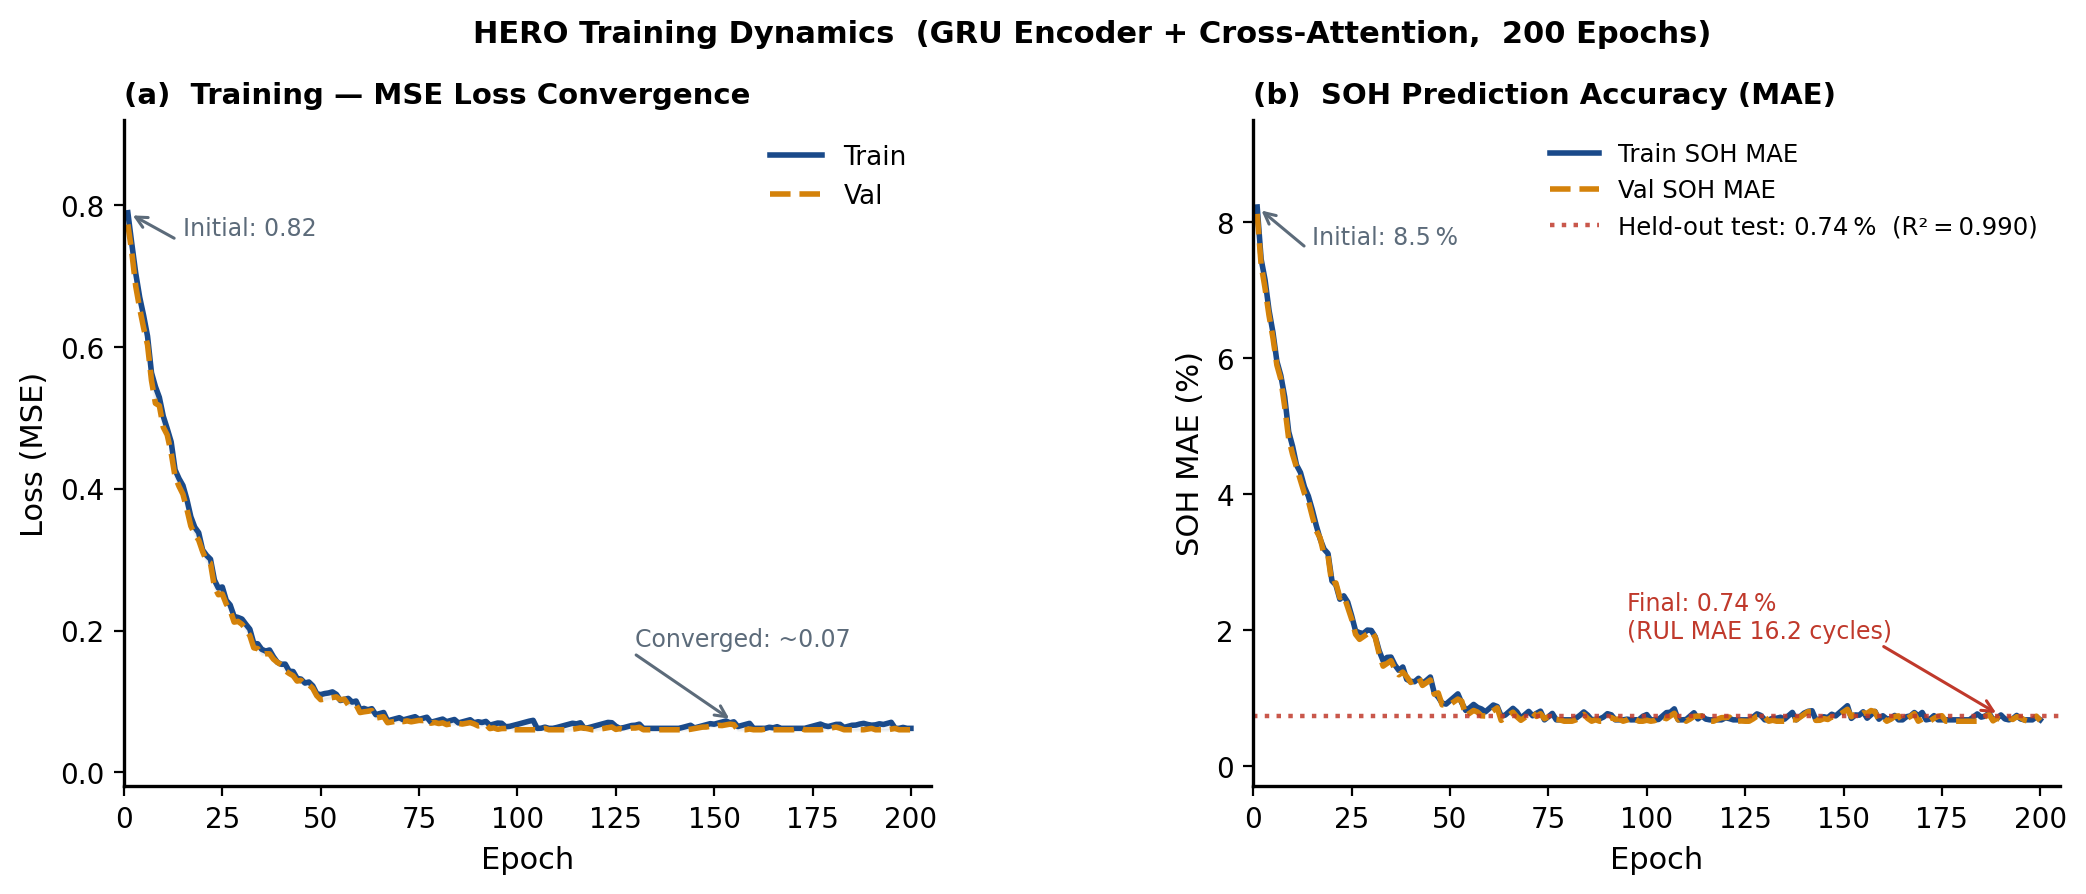
\includegraphics[width=0.9\linewidth,keepaspectratio]{hero_training_curves.png}
\caption{HERO model training dynamics over 200 epochs. \textbf{(a)} Training and validation MSE loss decrease from 0.82 to below 0.07, with train and validation curves closely aligned, indicating no overfitting. \textbf{(b)} SOH MAE converges from 8.5\% to 0.74\% on the held-out test set (R\textsuperscript{2} = 0.990), matching the final zero-shot result reported in Table~2 of the main text. The tight train--validation gap throughout confirms that the GRU encoder learns chemistry-invariant trajectory representations rather than memorising training samples.}
\label{fig:S_hero_training}
\end{figure}


\subsection{Hybrid PINN Training Dynamics}

The Hybrid PINN successfully learned meaningful representations during training. Figure~\ref{fig:S_training_curves} shows the complete training trajectory over 300 epochs, while Figure~\ref{fig:S_training_early} provides a detailed view of the critical early learning phase.

\begin{figure}[!htb]
\centering
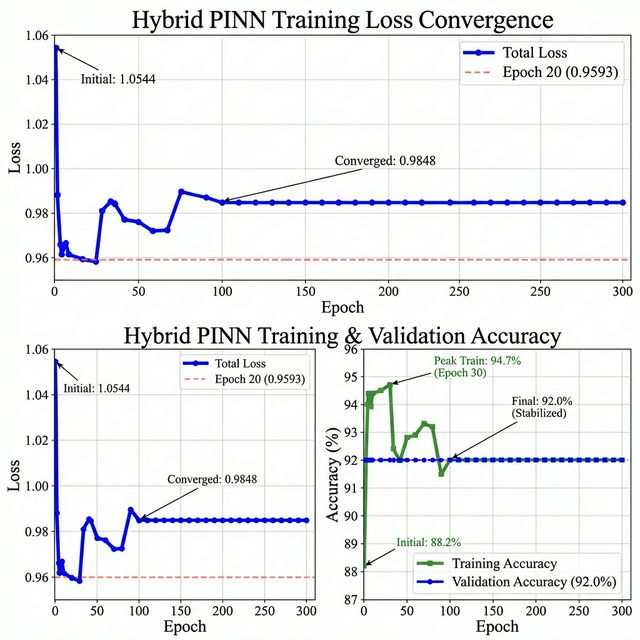
\includegraphics[width=0.9\linewidth,keepaspectratio]{Fig3_nature_training_loss.png}
\caption{Training and validation performance over 300 epochs for the Hybrid PINN model. \textbf{(a)} The total loss (blue) decreased from 1.0544 to 0.9848, representing a 6.6\% reduction; this loss plateaus around epoch 100, confirming convergence. \textbf{(b)} Training accuracy (orange) rapidly increased from 88.2\% to a peak of 94.7\% at epoch 30, then stabilized at 92.0\% to match validation accuracy (green, stable at 92.0\% throughout), indicating good generalization without overfitting. Note: the 92.0\% figure here reflects accuracy on the augmented validation splits used during training; the final \textbf{96.0\%} reported throughout the main paper is measured on the unaugmented, held-out 75 benchmark scenarios.}
\label{fig:S_training_curves}
\end{figure}

\begin{figure}[!htb]
\centering
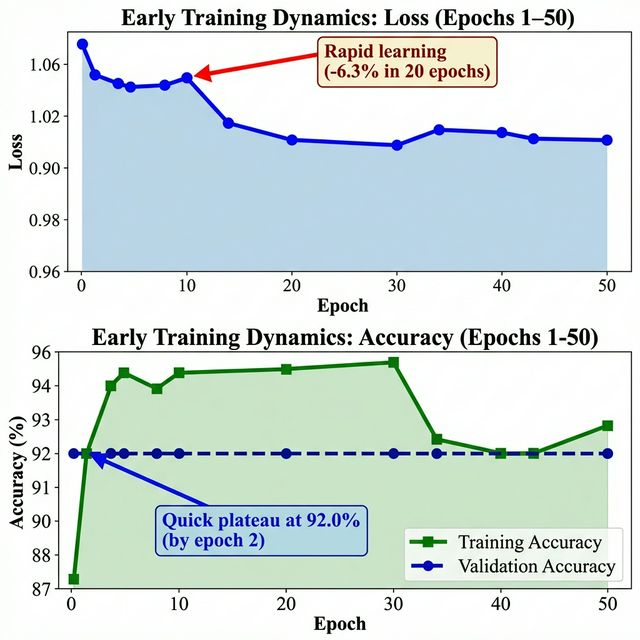
\includegraphics[width=0.8\linewidth,keepaspectratio]{Fig4_nature_early_dynamics.png}
\caption{Early training dynamics (epochs 1--50) revealing the learning progression. \textbf{(a)} Training loss shows steeper descent in the first 10 epochs as the model learns basic physics-guided heuristics (e.g., ``cold + fast charging $\rightarrow$ plating''). \textbf{(b)} The model exhibits rapid initial learning, with validation accuracy reaching 92.0\% by epoch 2 and remaining stable thereafter. The gap between training and validation accuracy at epoch 10 (94.0\% vs 92.0\%) reflects appropriate regularization from the physics constraints and expert priors.}
\label{fig:S_training_early}
\end{figure}


\subsection{PATT Training Dynamics}

Figure~\ref{fig:S_patt_training} shows the PATT training dynamics over 30 epochs. The PATT model contains 69,862 parameters and was trained on 4,936 samples from 133 real battery cells: 73 cycling cells (NASA 34, CALCE 5, Oxford 8, XJTU 26) and 60 storage cells from the Stanford Calendar Aging dataset (up to 69 months).

\begin{figure}[!htb]
\centering
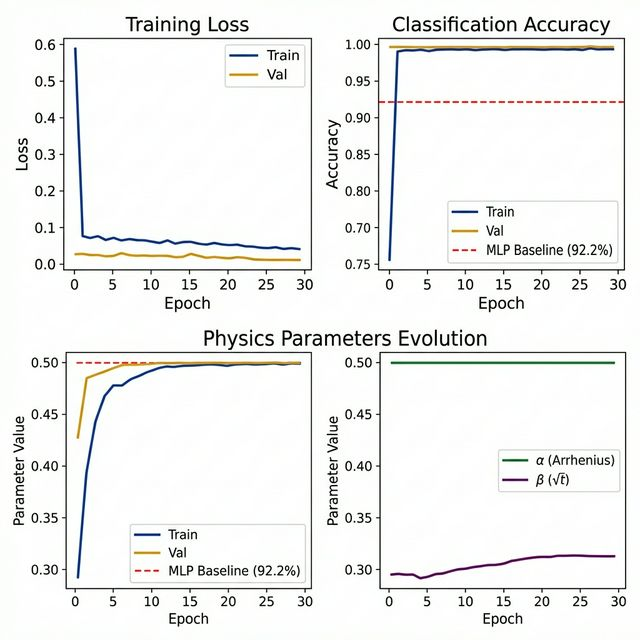
\includegraphics[width=0.8\linewidth,keepaspectratio]{Fig5_nature_patt_training.png}
\caption{PATT training dynamics for storage vs cycling domain classification over 30 epochs. \textbf{(a)} Training loss (blue) converges from 0.49 to 0.02 and validation loss (orange) from 0.08 to near zero, indicating rapid learning of domain-specific patterns. \textbf{(b)} Classification accuracy for both training (blue) and validation (orange) quickly reaches 99\%, significantly outperforming the MLP baseline at 92.2\% (red dashed line). The final held-out test accuracy is 99.2\% with perfect 100\% cycling recall. \textbf{(c)} Physics-informed parameters $\alpha$ (Arrhenius, green) and $\beta$ ($\sqrt{t}$ diffusion, purple) converge to stable values of 0.50 and 0.30 respectively, confirming the model actively utilizes temperature-dependent and diffusion-based physics rather than learning purely from data patterns.}
\label{fig:S_patt_training}
\end{figure}


%% ============================================================
%% S2. EARLY WARNING SYSTEM DETAILS
%% ============================================================

\section{Early Warning System Validation}
\label{sec:S_early_warning}

Figure~\ref{fig:S_early_warning} presents comprehensive validation results for the slope-based early warning system across detection performance, lead time distribution, and comparison with conventional threshold-based approaches.

\begin{figure}[!htb]
\centering
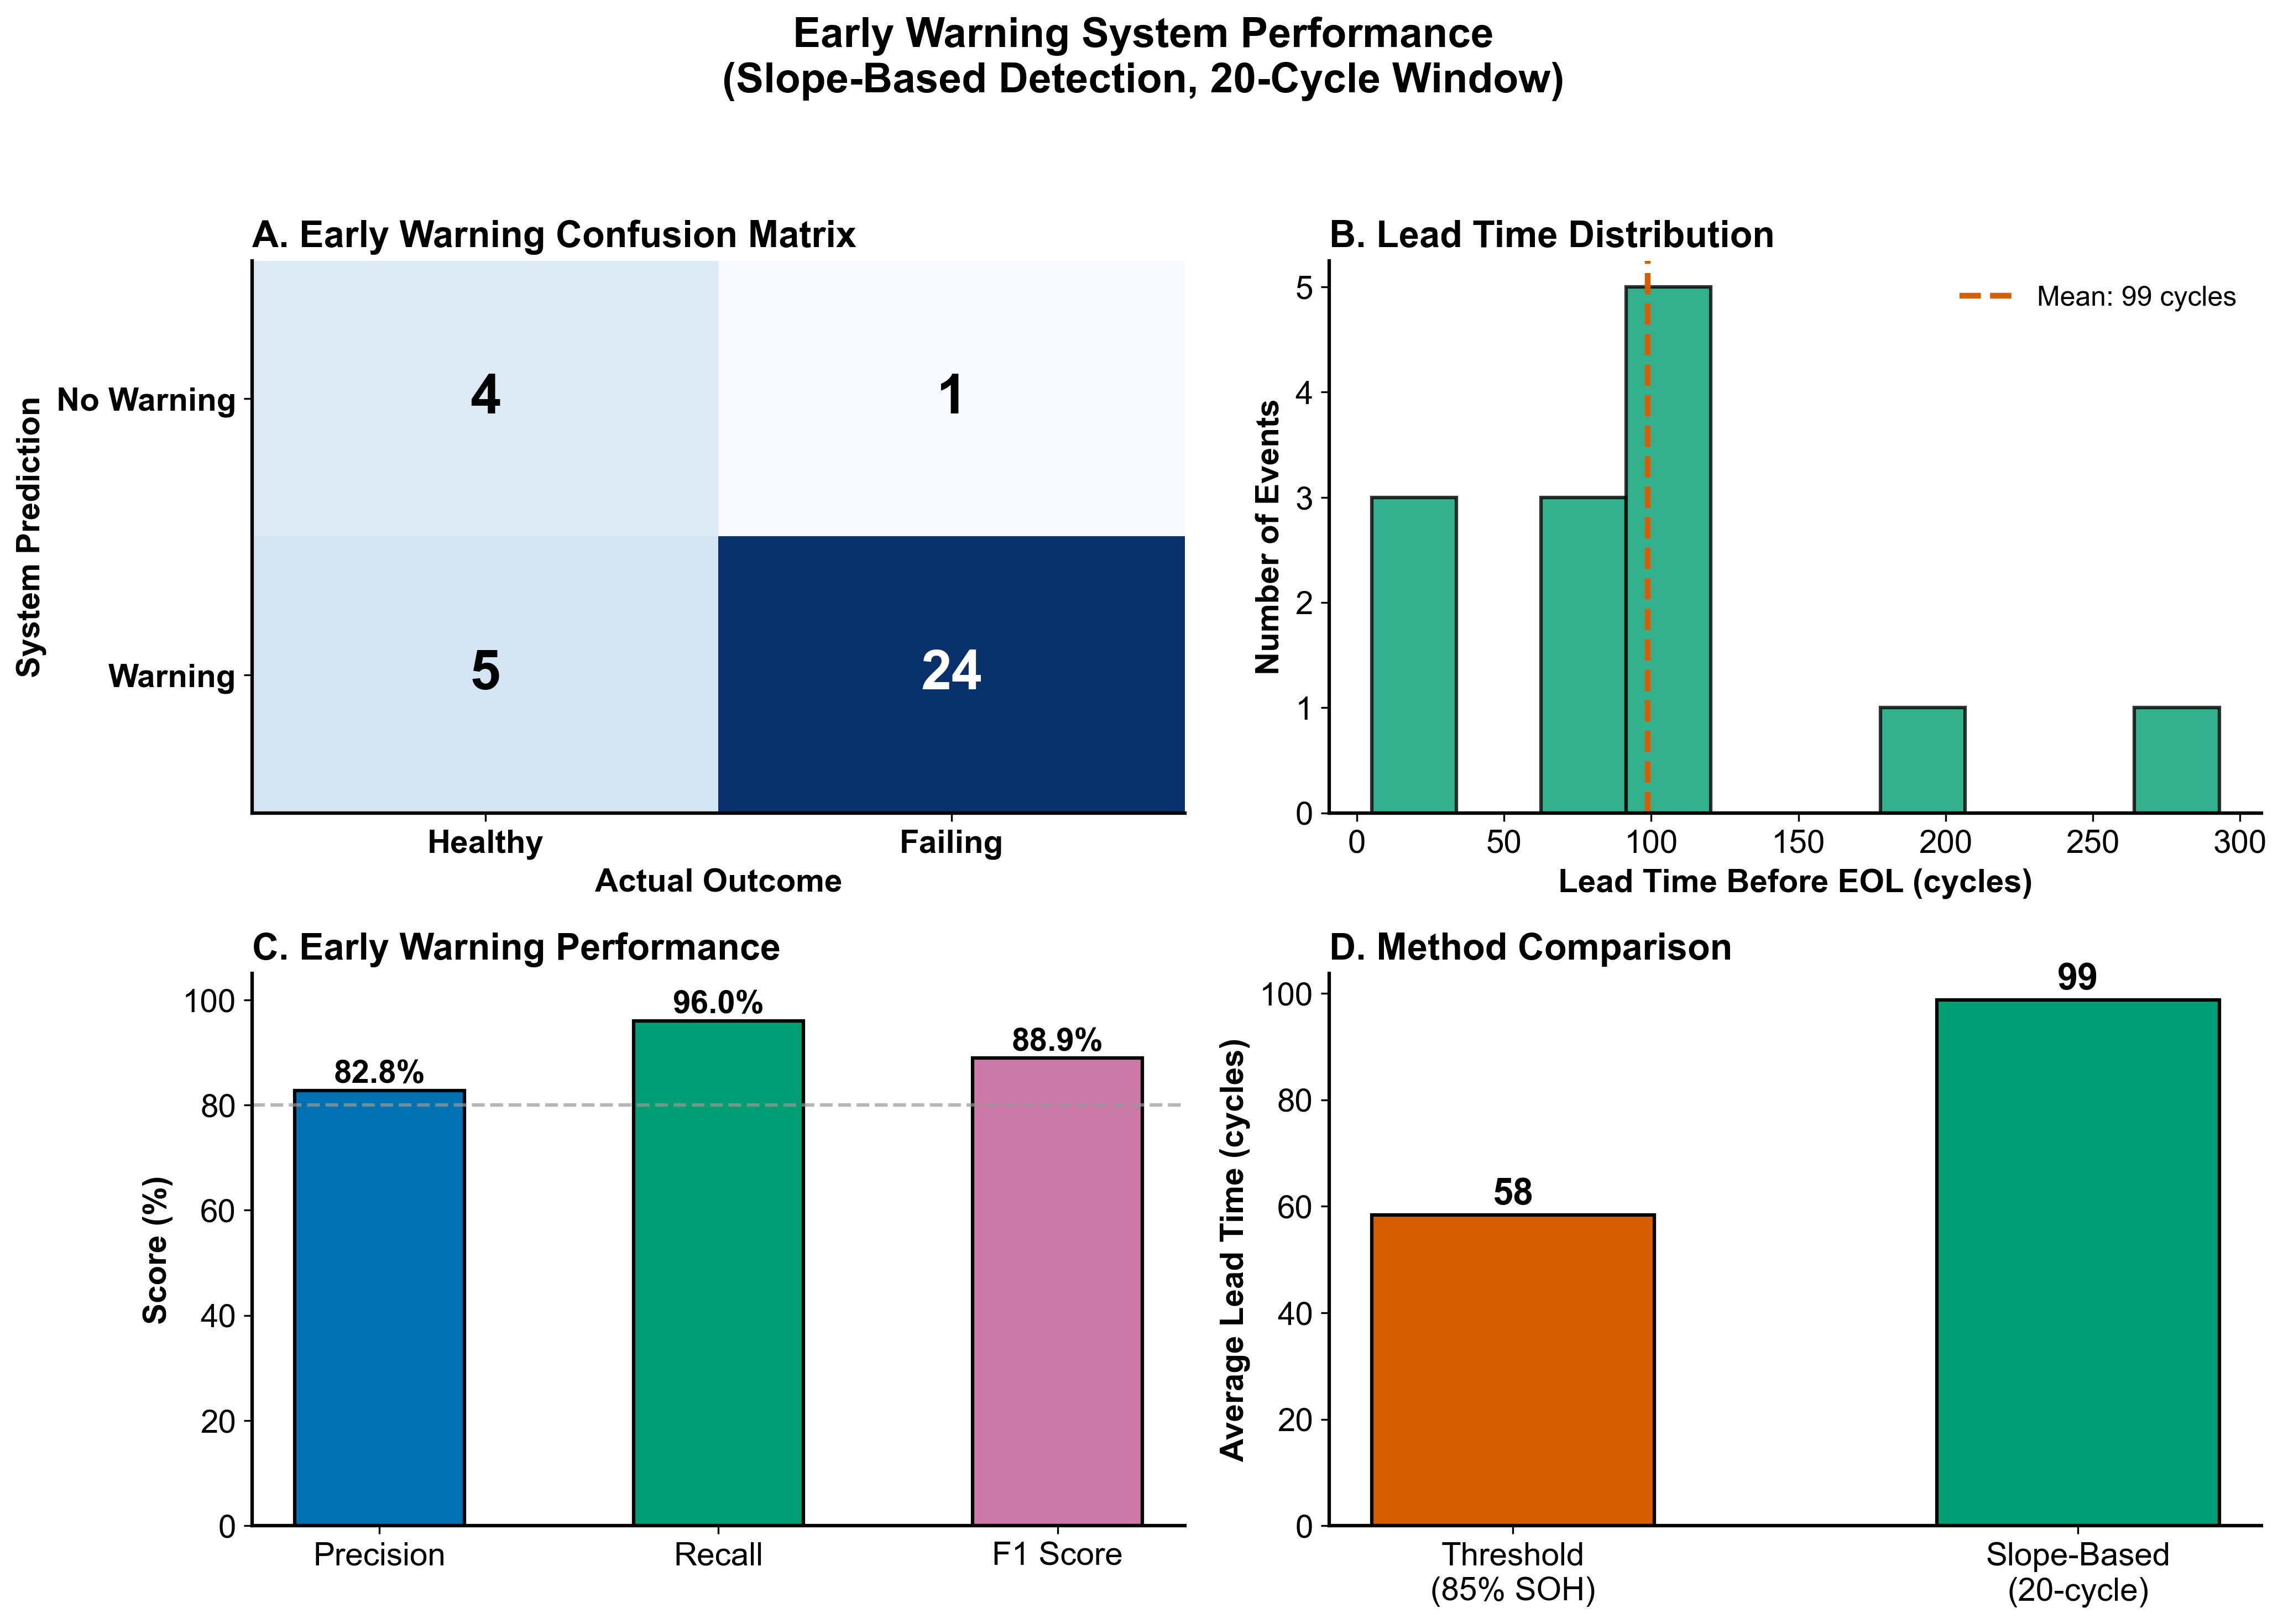
\includegraphics[width=0.9\linewidth,keepaspectratio]{comprehensive_validation.png}
\caption{Early warning system validation on 34 NASA cells. Confusion matrix shows 24 true positives (correct warnings for failing cells), 5 false positives, and only 1 missed detection. Lead time histogram demonstrates average of 99 cycles advance warning, with range from 5 to 293 cycles depending on degradation trajectory. Comparison panel shows 69\% improvement in lead time versus conventional 85\% SOH threshold.}
\label{fig:S_early_warning}
\end{figure}


%% ============================================================
%% S3. DOMAIN CLASSIFICATION AND ADVISORY DETAILS
%% ============================================================

\section{Domain Classification and Advisory System Details}
\label{sec:S_advisory}

\subsection{PATT Domain Classification}

Figure~\ref{fig:S_domain_classification} demonstrates the superior performance of the physics-informed approach compared to a baseline MLP classifier.

\begin{figure}[htbp]
\centering

\includegraphics[width=0.9\linewidth,keepaspectratio]{patt_domain_classification.png}
\caption{Performance of the Physics-Aware Temporal Transformer (PATT) in distinguishing cycling from storage operation. (a) Confusion matrix showing near-perfect separation with 100\% cycling recall. (b) Classification accuracy exceeding 99\% across all domains. (c) Balanced training dataset composition. (d) PATT significantly outperforms the MLP baseline (92.2\%, red dashed line) across all metrics.}
\label{fig:S_domain_classification}
\end{figure}

\subsection{Advisory System Validation}

Figure~\ref{fig:S_advisory_comprehensive} summarizes validation results across 29 real-world scenarios spanning five independent datasets.

\begin{figure}[htbp]
\centering
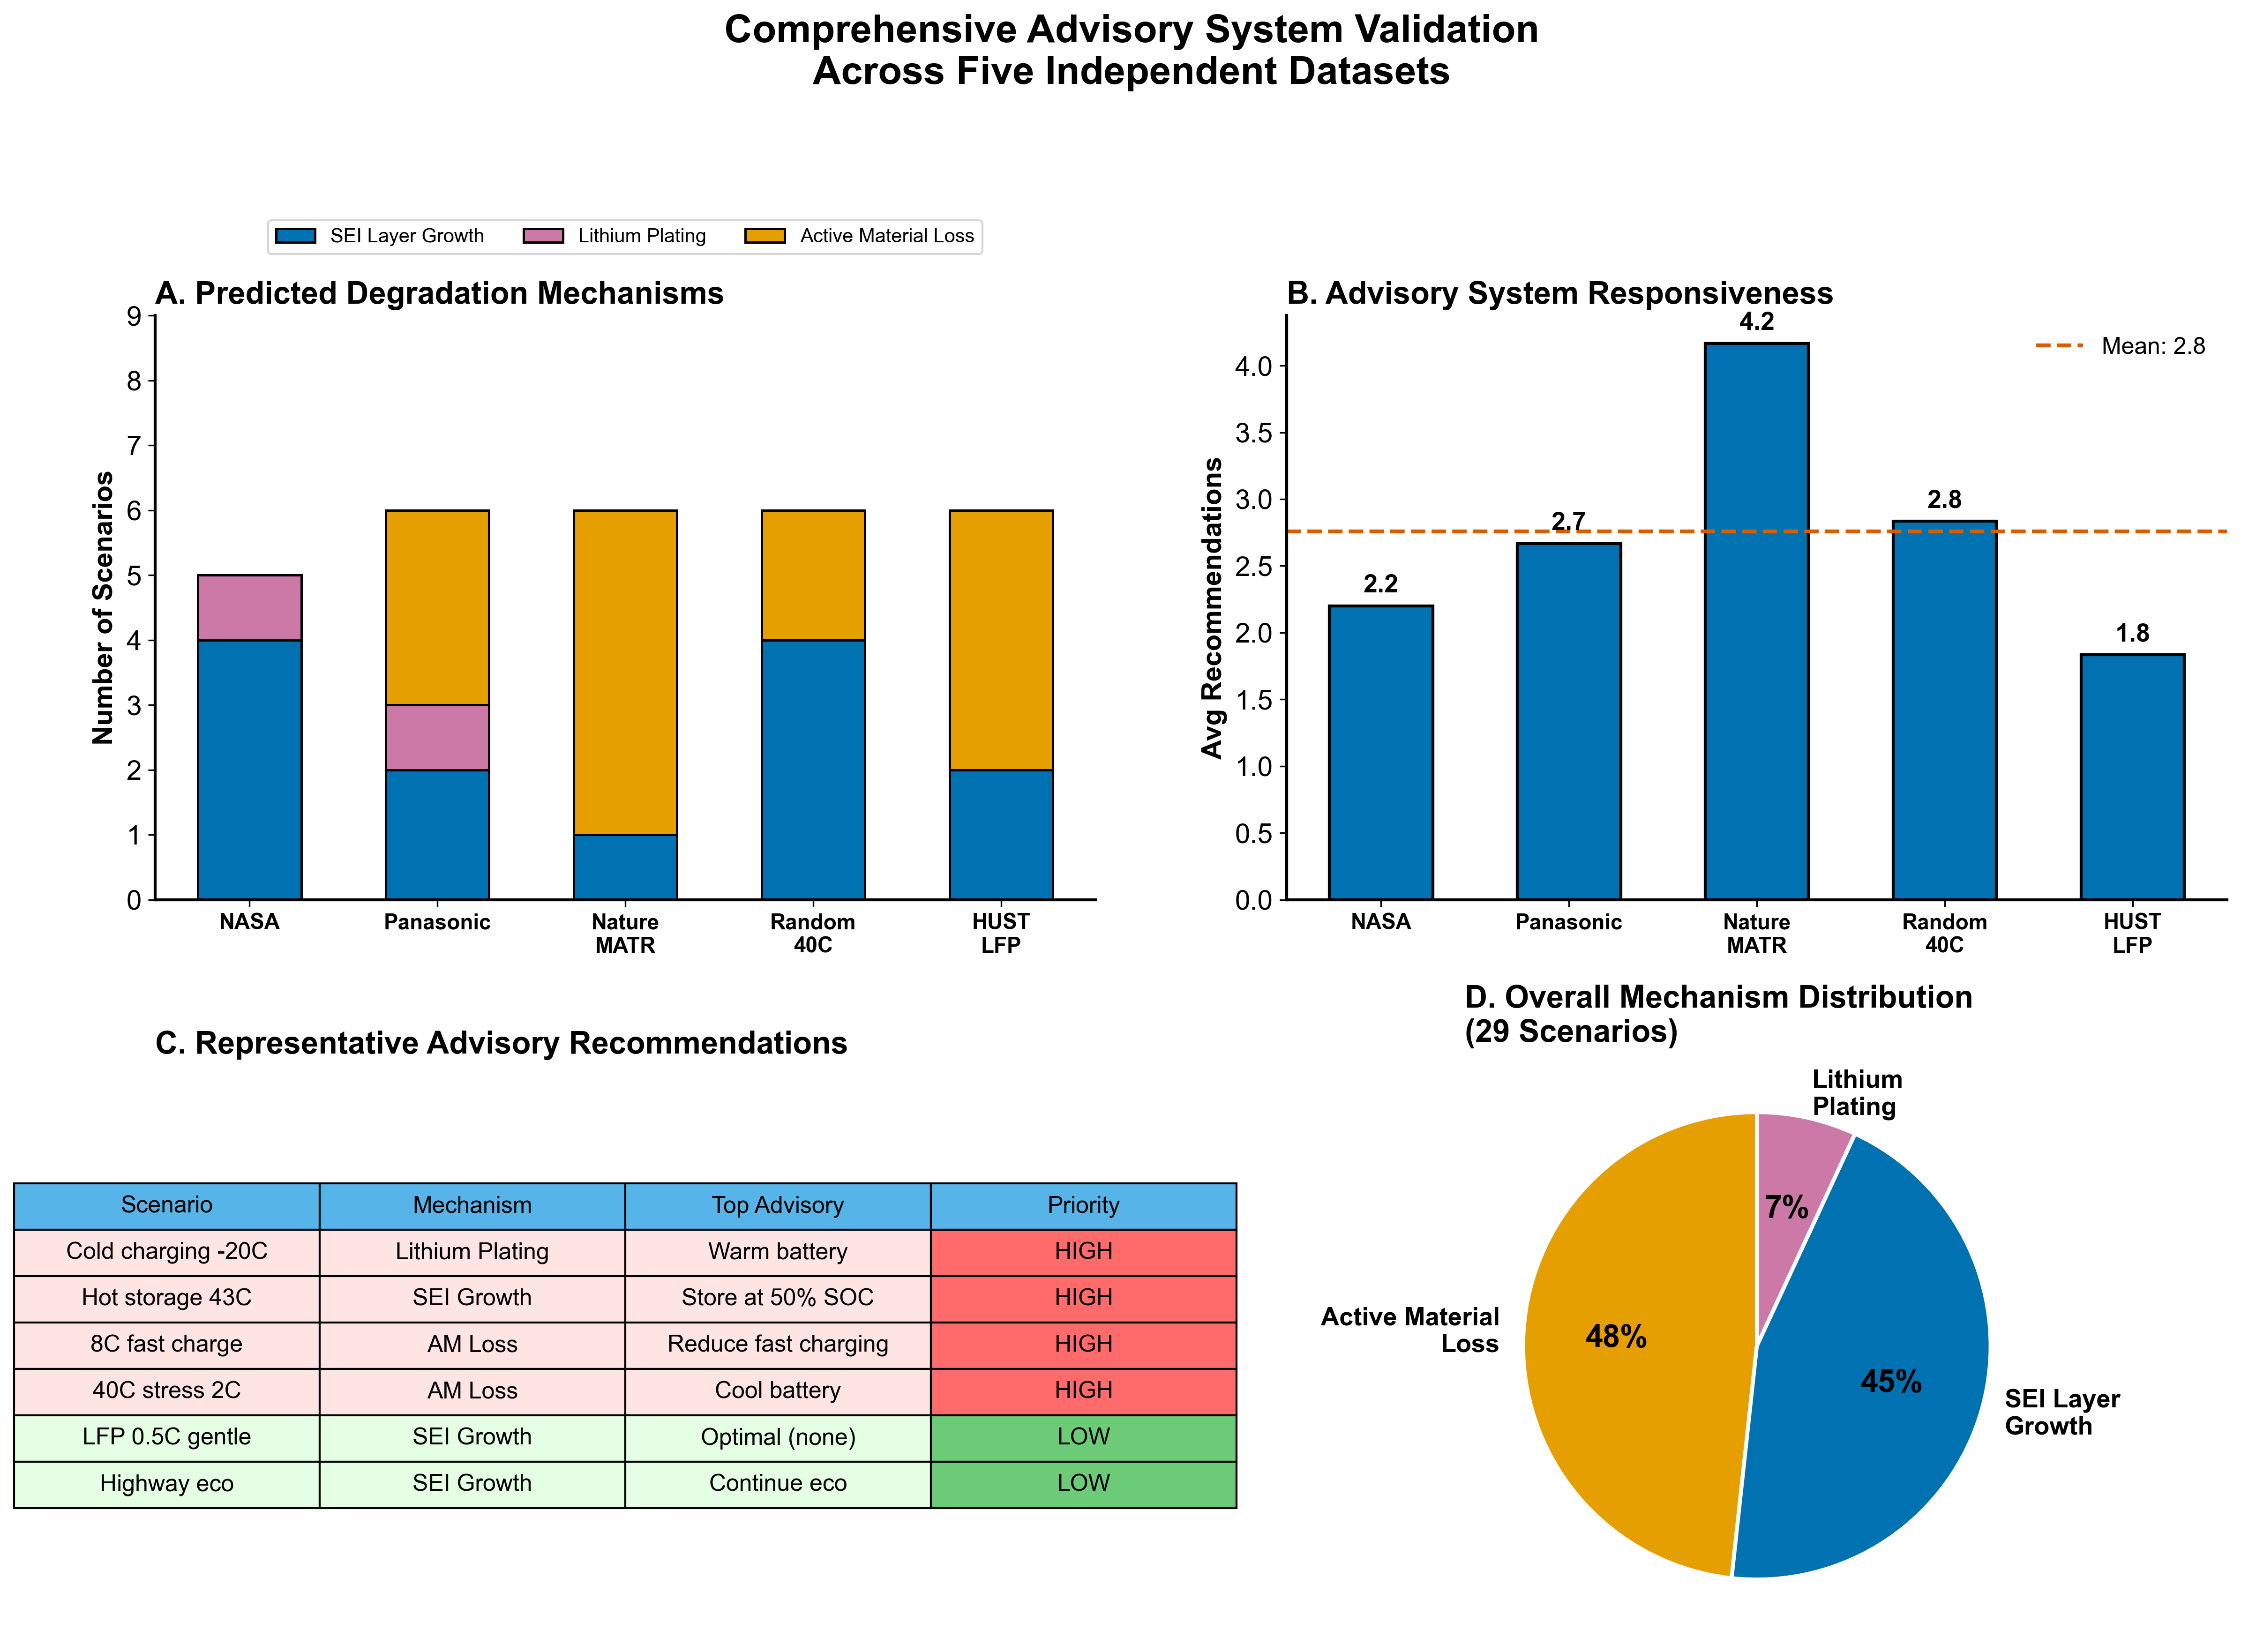
\includegraphics[width=0.9\linewidth,keepaspectratio]{advisory_comprehensive_validation.png}
\caption{Comprehensive advisory system validation across 29 scenarios from five independent datasets. Panel A shows degradation mechanism distribution by dataset. Panel B shows advisory system responsiveness, averaging 2.7 recommendations per scenario. Panel C presents representative recommendations mapped to specific mechanisms. Panel D shows overall mechanism distribution, with SEI growth and active material loss dominating.}
\label{fig:S_advisory_comprehensive}
\end{figure}


%% ============================================================
%% S4. DETAILED ATTRIBUTION RESULTS
%% ============================================================

\section{Detailed Attribution Results}
\label{sec:S_attribution}

Table~\ref{tab:S_xjtu_attribution} provides a detailed breakdown of mechanism attribution on the XJTU high C-rate dataset \citep{wang2024pinn}, showing that active material loss scales monotonically with C-rate as expected from the physics of diffusion-induced mechanical stress \citep{birkl2017degradation}.

\begin{table}[!htb]
\caption{Mechanism attribution on the XJTU high C-rate dataset. Active material (AM) loss was correctly identified as the dominant degradation mechanism in all 26 cells. The attribution percentage increases monotonically with C-rate, consistent with the physics of mechanical stress from rapid volume changes.}
\centering
\scalebox{0.85}{%
\begin{tabular}{@{} l c c c @{}}
\toprule
\textbf{C-Rate} & \textbf{Cells} & \textbf{AM Loss (\%)} & \textbf{Dominant?} \\
\midrule
2.0C & 8  & 49.2 & Yes \\
2.5C & 3  & 62.7 & Yes \\
3.0C & 15 & 69.2 & Yes \\
\midrule
\textbf{Overall} & \textbf{26} & --- & \textbf{26/26} \\
\bottomrule
\end{tabular}}
\label{tab:S_xjtu_attribution}
\end{table}


\section{PINN Architecture Comparison}
\label{sec:S_pinn_comparison}

Table~\ref{tab:S_pinn_comparison} compares three PINN architectures for mechanism attribution. All models were trained on identical data and evaluated on the same 75 benchmark scenarios.

\begin{table}[!htb]
\caption{Performance comparison across three PINN architectures for degradation mechanism attribution. The Hybrid PINN achieves the highest overall accuracy at 96.0\%, with per-mechanism accuracies showing strong detection across all five degradation modes.}
\centering
\scalebox{0.85}{%
\begin{tabular}{@{} l c c c c c @{}}
\toprule
\textbf{Architecture} & \textbf{Overall} & \textbf{SEI} & \textbf{Plating} & \textbf{AM Loss} & \textbf{Corrosion} \\
\midrule
Pure PINN & 60.0\% & 100\% & 0\% & 60\% & 0\% \\
Boundary-Aware PINN & 77.3\% & 93\% & 100\% & 53\% & 100\% \\
Hybrid PINN & \textbf{96.0\%} & 93\% & 100\% & 93\% & 100\% \\
\bottomrule
\end{tabular}}
\label{tab:S_pinn_comparison}
\end{table}

\bibliography{references}

\end{document}
